\section{DAQ} \label{sec:daq}

This section outlines the data acquisition system for ProtoDUNE.
The DAQ system is shown in figure \ref{fig:daq-overview} along with its
interfaces to the cold electronics, beam instrumentation, and online
computing systems.


\begin{cdrfigure}[DAQ Overview]{daq-overview}{Detailed overview of the
DAQ system, its interconnections, data flow, timing and control signals,
and the interfaces to the electronics and online computing systems
\fixme{simplify diagram for TDR}}
        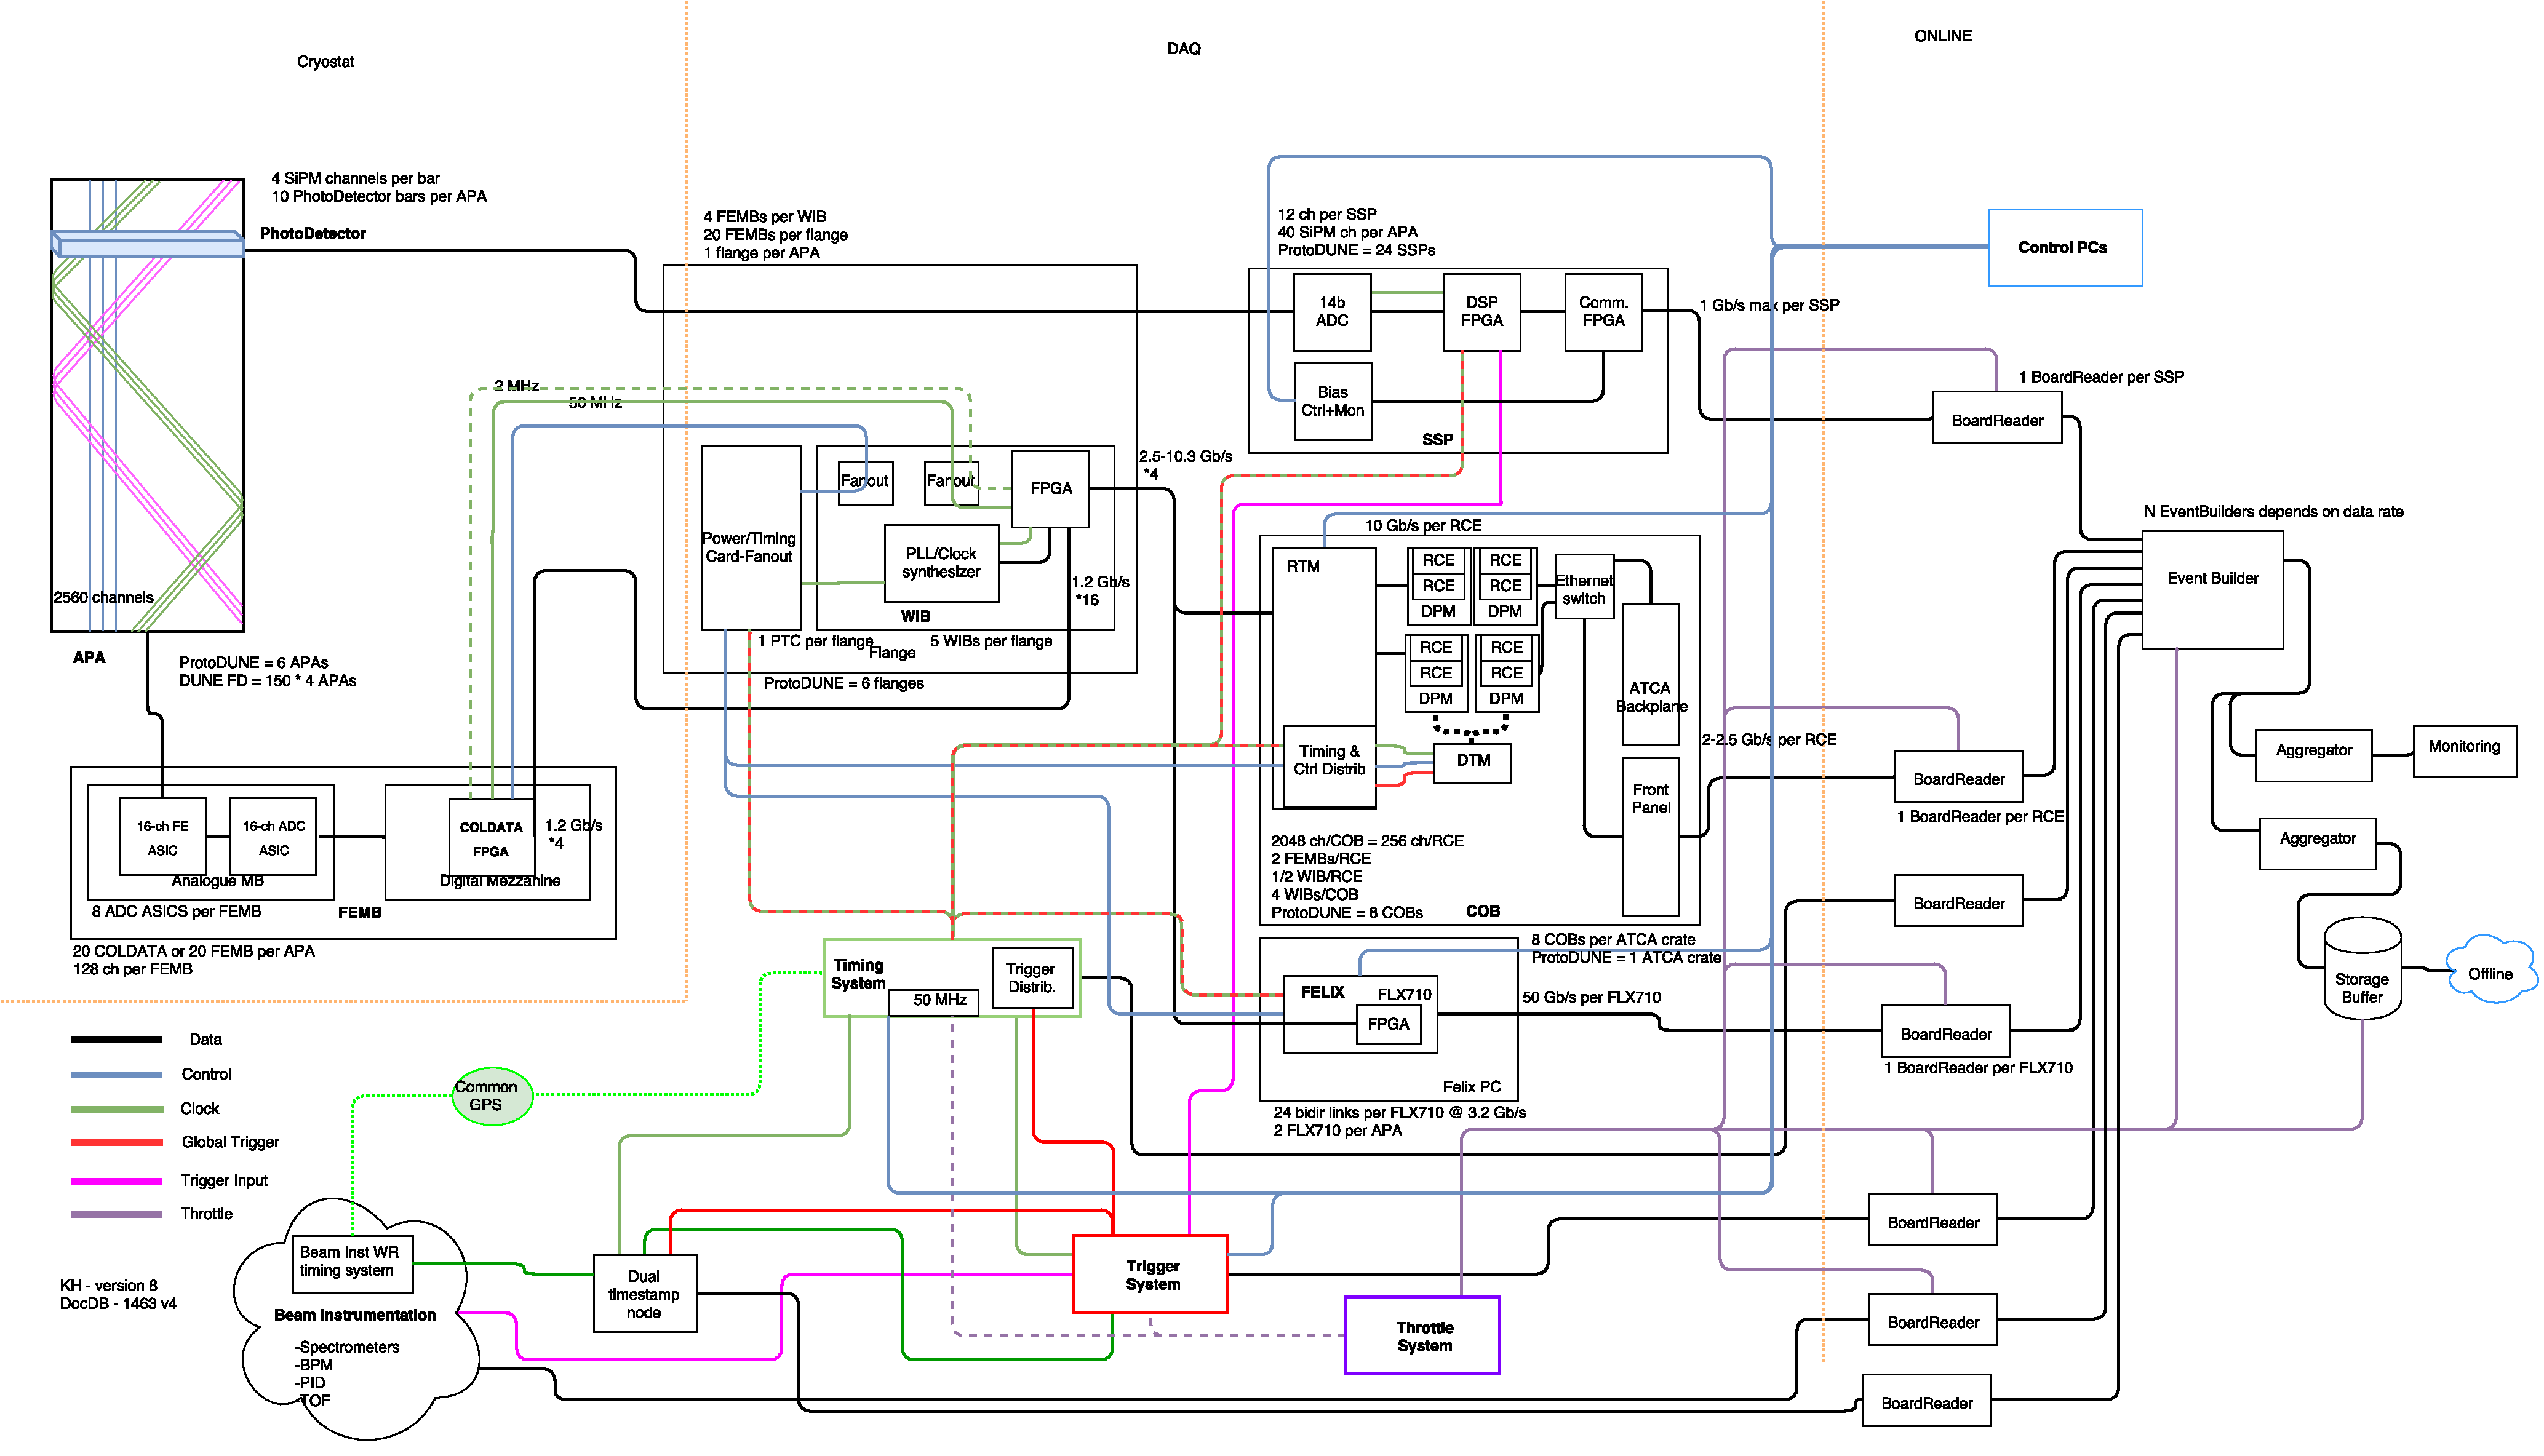
\includegraphics[angle=90,width=0.70\textwidth]{daq-overview-dia.pdf}
\end{cdrfigure}

%%%%%%%%%%%%%%%%%%%%%%%%%%%%%%%%%%%%%%%%%%%%%% \subsection{Introduction}

%\emph{GB:}

%Brief overview of requirements for the collection of data for the
%primary goals.  (what subdetectors exist (TPC, PDS, trigger, beam
%counter monitoring, is there a beam position monitor (wire chamber or
%fiber detetor in the beam), a cosmic veto, a beam halo veto?  If so,
%who is doing these things?), primary readout scheme, alternative readout
%schemes including FELIX (section~\ref{ssec:daqfelix}) what the data rates
%are for the beam, need for calibration etc.).  Description of modes of
%operation (triggered, extended test modes for far detector).

%Overview of how the DAQ will be commissioned (importance of online monitor
%early (and therefore need early definition of data format and simulation).

%Diagram: Physical connections between the main modules, showing the RCEs,
%FELIX, SSPs, and some generic beam detector readout.  Show timing system
%and show exiting arrows for where data are feeding the slow control.
%Have the offline as a generic blob (i.e. details of data distribution
%are in a different section)

%Descrine the above diagram.  Give table of rates in each branch, and make
%the comments on the data rates (i.e. anticipate questions the reviewers
%may have about bottlenecks).


The requirements for the DAQ system for ProtoDUNE are defined
by the physics requirements of the experiment, with constraints from the
front-end electronics and assumed bandwidth and storage requirements
from the online and offline computing systems.  The baseline trigger
rate during the SPS spill is taken to be 25 Hz.  Cosmic data will also
be acquired at a rate of approximately one third of the beam rate.

The data rate from the electronics is assumed to be dominated by the
TPC data.  However, the photon detection system may be a significant
bandwidth contribution, particularly when reading out calibration data
(where full waveforms are extracted).  \fixme{need real numbers for SSPs}.
The TPC data is sent via the Warm Interface Boards on the cryostat flanges
for the six APAs of ProtoDUNE un-triggered at a total rate of 491.52 Gb/s
(6 APAs $\times$ 2560 channels $\times$ 16 bit ADC $\times$ 2 MHz).
ProtoDUNE will have 24 SSPs reading out the Photon Detection System at
a maximum rate of 1 Gb/s each.

The maximum bandwidth from the ProtoDUNE online system to CERN IT (and
hence, the offline world), is considered to be 20 Gb/s at a maximum.
Therefore, the DAQ system must reduce the data by a significant fraction
before the data is sent offline.  This is achieved by a combination of
data compression and triggering.

%%%%%%%%%%%%%%%%%%%%%%%%%%%%%%%%%%%%%%%%%%%%%%

%%%%%%%%%%%%%%%%%%%%%%%%%%%%%%%%%%%%%%%%%%%%%% 
\subsection{Timing and Trigger}
\label{sec:daq_time}

The timing and the trigger are two distinct subsystems.  The timing
system provides the distribution for the trigger signals over the same
fabric as the clock and calibration signals.  Each of the systems will
be described separately, along with a brief section on the interface to
the beam instrumentation.

\subsubsection{Timing}


The timing system is required to: provide a stable and phase-aligned
master clock to all DAQ components; synchronize external signals into the
ProtoDUNE clock domain and time-stamp them; distribute synchronization,
trigger and calibration commands to the DAQ system; and conduct continuous
checks of its own function. In addition, the timing system acts as a
data source, providing a record of triggers received, distributed, or
throttled. The system is designed to meet the full eventual requirements
of the DUNE experiment, but will need only a subset of that functionality
for ProtoDUNE. For instance, absolute time-stamping with respect to an
external GPS reference is not required, nor is the partitioning of the
experiment into independent timing zones.

An FPGA-based master unit receives a high-quality clock (provided in
ProtoDUNE by a quartz crystal oscillator) and external signals from the
trigger system and SPS accelerator. It interfaces to the ProtoDUNE control
and DAQ via a gigabit Ethernet interface. The master unit multiplexes
synchronization and trigger commands, along with arbitrary command
sequences requested by software, into a single encoded data stream,
which is broadcast to all timing endpoints, and decoded into separate clock
and data signals. A uniform phase-aligned cycle counter, updating at the
ProtoDUNE system frequency of 50MHz, is maintained at all endpoints,
allowing commands to take effect simultaneously at all endpoints
regardless of cable lengths or other phase delays.

The timing signal is broadcast via multi-mode optical fiber (for
medium-distance connection to the WIB crates on the detector) and LVDS
signals over twisted pair cable (for short-distance connection to RCEs,
SSPs and FELIX modules). Optical signals are fanned out and recombined
using commercial 32:1 passive splitters, and active optical--LVDS
converter boards further split the signals for local distribution to
endpoints. The system uses duplex links, allowing all endpoints to be
regularly interrogated during system operation to ensure correct operation
and reception of timing commands. Along with the possibility to select
any given endpoint via a unique network address, this mechanism also
allows automatic phase-adjustment of all local clocks at system start-up,
through precise measurement of the returned clock phase at the master unit.

Endpoints decode the timing signal into separate clock and data
signals using a commercial clock-data recovery ASIC, which in turn
feeds a low-bandwidth PLL in order to remove any remaining jitter in
the clock and provide phase adjustment. The data stream employs 8b/10b
encoding, ensuring sufficient transitions in the timing signal for clock
recovery and correct operation of optical links, and uses scrambling
of idle patterns to minimise EMI. A common firmware block is used to
decode the timing protocol, which is incorporated into the overall
firmware design for the receiving FPGA in each DAQ component. This
block provides a cycle counter, several independent trigger, calibration and 
synchronisation signals, and a general-purpose packet data output to each endpoint.
The cycle counter may be used further to generate low-frequency timing signals for
further propagation, e.g. the 2MHz sampling signal for the cold ADCs.

\subsubsection{Trigger}

\fixme{Need to finalise group on this soon - possibly UPenn and others}

\subsubsection{Beam Interface}

The Beam Instrumention is described in section \ref{sec:beaminstruments}.

%%%%%%%%%%%%%%%%%%%%%%%%%%%%%%%%%%%%%%%%%%%%%% 
\subsection{TPC data readout}

\fixme{ 
        %\emph{GB:} 
        Present the RCE system - just the main data flow, merging,
compression etc.  State that the way the data are collected together,
timing system, control etc., will be handled in section~\ref{sec:daq},
sentence at the end to say that the architecture allows future
readout schemes to be incorporated and tested with ProtoDUNE and
that these will be discussed, in particular the FELIX system, in
subsection~\ref{ssec:daqfelix} }

The readout of the ProtoDUNE TPC wires, prior to being received by PCs in
the back-end DAQ, consists of the electronics directly attached the APAs,
inside the cryostat (the cold electronics) and the electronics outside
the cryostat, either directly on the cryostat flange or in a rack (the
warm electronics).  This proposal addresses the warm part of the TPC
readout and how it receives data from the cold electronics (the Front-End
Boards), manipulates the data, and delivers it to the back-end DAQ.

From an electronics point-of-view, the ProtoDUNE flange will consist of
5-slot ``crate'', where the connectors on the warm side of the feed
through form the ``back-plane'' into which the boards plug when inserted
into the ``crate'' assembly.  These connectors and the boards that plug
into the ``crate'' assembly.  These connectors and the boards that plug
into them (the WIBs, or warm interface boards) serve to send the power,
timing, and configuration down to the FEBs and receive the high-speed
signals from the FEBs. From a data standpoint, each WIB receives the
data from 4 FEBs, over sixteen 1.25-Gbps data lines, and multiplexes
this data to four 5-Gbps (or two 10 Gbps) lines which are sent over
optical fiber the DAQ.

Two systems will be used to receive data from the WIBs.  The baseline
solution is based on Reconfigurable Computing Elements (RCE) and will
readout data from 5 APAs.  An alternative exploratory prototype based on
the Front-End-Link-EXchange (FELIX) system will be used to readout 1 APA.

\subsubsection{RCE based readout}
The data from the WIB are received by processing units called RCEs
(Reconfigurable Computing Elements), which are housed in industry-standard
ATCA shelves on COB (cluster-on-board) motherboards that are designed
at SLAC for a wide range of applications.   The RCE is a SoC from the
Xilinx Zynq family and contain a full Linux processor system on the chip
accompanied by 1 GByte of DRAM.   The primary processing function of the
RCEs for ProtoDUNE are compression (or zero-suppression) and buffering
of the raw data and then sending data to the back-end upon the receipt of
an external trigger.  Each COB carries 8 RCEs, each connected to each
other via an on-board 10 Gbps Ethernet switch which also sends data out
of the COB the back-end DAQ PCs.

The interface with the WIB is provided via the ATCA compliant rear-board
(the RTM=Rear Transition Module).  This is an application-specific board
that is custom made depending on the physical characteristics of the
connections to-and-from the FE (e.g. fiber or electrical connections,
number and types of transceivers, timing \& trigger connections, etc).
For ProtoDUNE, the RTM will use a set of QSFP transceivers to receive
the data from the WIB and an SFP+ optical interface for communication
with the timing and trigger distribution system.

As the multiplexed data from the WIB comes into the RCE FPGA fabric
it will be de-multiplexed and buffered into per-channel, fixed-time
length chunks (for instance 512- or 1024-ticks).  These chunks will be
compressed and written to the DRAM where the RCE processor will wait
for a trigger (also handled by the FPGA) to arrive.  Upon a trigger, the
processor will sends a fixed number of pre- and post-trigger time chunks,
for all channels, to the back-end PCs.  Apart from the compression step,
this design is very similar to that used on the 35ton prototype DAQ.

For ProtoDUNE, 256-wires worth of data (2 FEBs) will be sent to each RCE.
Given that there are 120 FEBs in ProtoDUNE, 60 RCEs will be needed to
readout the full detector.  These will fits into 8 COBs which in turn
will reside in a single 14-slot ATCA shelf.

\subsubsection{FELIX based readout}
The FELIX is a PCIe card receiving data on point-to-point links from
the detector electronics and routing those through a switched network
to computers.  The aim is to reduce to a minimum any specific hardware
developments and to fully rely on commercial networks and servers to
perform the DAQ tasks.  For ProtoDUNE data from 5 WIBs (20 FEBs) will
be readout over ten 9.6 Gbps links into two FELIX cards.  Grouping
time-slices around a trigger signal, as well as data compression will be
dealt with in software. Similar to the RCE based readout the FELIX will
generate artDAQ fragments to be sent to the event builder.


%%%%%%%%%%%%%%%%%%%%%%%%%%%%%%%%%%%%%%%%%%%%%% 
\subsection{PDS data readout}

\fixme{The photon people like consider the SSPs as
electronics, not DAQ, so that may all be in the photon section - KH}

%%%%%%%%%%%%%%%%%%%%%%%%%%%%%%%%%%%%%%%%%%%%%% 
\subsubsection{Beam instrumentation readout}

\fixme{
When groups are known, describe how integration of beam counter
monitoring, beam position monitors (wire chambers of fibre detectors in
the beam to measure position and improve momentum resolution) will be
done. also cosmic veto or halo veto around beam.   For the beam counter
monitoring, it may be that the 35t Penn trigger board could be used.
}


%%%%%%%%%%%%%%%%%%%%%%%%%%%%%%%%%%%%%%%%%%%%%% 
\subsection{Event building software }

\fixme{ %\emph{KH:}
        artDAQ is briefly described in section~\ref{sec:DAQ_online_interface}
but I think we need it in more detail here.  By contrast the online
computing infrastructure should be left for the computing section.

%\emph{GB:}

Describe artDAQ, data handling capabilities, current plans, extensions
foreseen for final DUNE, throughput tests already made and planned.
Control of artDAQ processes (DAQIFACE), error handling, debugging
emulation mode.  }

%%%%%%%%%%%%%%%%%%%%%%%%%%%%%%%%%%%%%%%%%%%%%% 
\subsection{Software filtering and data transfer to permanent storage}

\fixme{
        \emph{KH:} Compare this to the computing section and find where
        best to implement. \emph{GB:} Point out that compression and/or
        further event sorting can
be done in either the artDAQ trigger farm, or the online computing farm
(run by the S\&C group).  Describe where we are on this (i.e. what
compression algorithms, etc.  experience from other experiments).
Describe how the hand-off to the S\&C processes writing to permanent
storage work. Address the question of disk writing speeds.
}


%%%%%%%%%%%%%%%%%%%%%%%%%%%%%%%%%%%%%%%%%%%%%% 
\subsection{Control, configuration and operational monitoring}
The artDAQ software used for all applications dealing with the movement,
processing and storage of data will be interfaced with software of the
Joint Controls Project (JCOP) for the purpose of control, configuration
and operational monitoring.  JCOP provides a toolkit to implement run
control (finite state machine (FSM), distribution of commands, error
propagation and handling) as well as graphics tools that allow for the
implementation of user interfaces and monitoring dashboards.  In order to
minimize the software development needs the same FSM as defined by artDAQ
will be implemented and commands will be sent to the applications using
the already supported XML-RPC protocol.  Monitoring data will be pushed
into the JCOP framework by implementing the appropriate artDAQ monitoring
plugin.  Log and error messages will be most probably collected and
processed using an implementation of the ELK (elastic search, logstash,
kibana) stack.  The internal configuration of DAQ applications will be
carried out using the mechanisms provided by artDAQ. The overall system
will be modeled and configured using the JCOP paradigm (data points).

%\fixme{\emph{KH:} Requires some more discussions on the run control software
%        choices,  artDAQ, WinCC/JCOP etc.
%\emph{GB:} (a.k.a. run control) [Before writing,
%it would be good to clarify the relationship between the two options
%(1) Erik Blaufuss's ICECUBE philosophy to put all run conrol into one
%browser interface with one authentication point, which is excellent
%and (2) either CERN WIN-xx or EPICS/CAA uBooNE system which are off
%the shelf environments.   How to decide - want biggest team of people
%with >30\%fTE + commitment to be at CERN for ~3months over next 2 years,
%and then let them decide]}


\subsection{Data quality monitoring}
In addition to the monitoring of the operations of the DAQ system, the
quality of the data taken by the detectors has to be constantly monitored.

\fixme{Here describe the online and nearline monitoring frameworks and
a non-exhaustive list of what is being monitored.  Who will write this?}

%%%%%%%%%%%%%%%%%%%%%%%%%%%%%%%%%%%%%%%%%%%%%% 
%\subsubsection{Alternative readouts - FELIX} \label{ssec:daqfelix}

%\fixme{
%Short paragraph saying that alternative readouts can be tested by
%replacing or adapting the WIBs to feed new systems.  A particular
%development which we want to persue vigerously is the FELIX system
%developed by a consortium incluing CERN, BNL, NIKHEF for ATLAS and for
%which all of these groups and PNNL are persuing for DUNE.   However, it
%is not a requirement that this readout is operating on day 1 of ProtoDUNE.
%}

%%%%%%%%%%%%%%%%%%%%%%%%%%%%%%%%%%%%%%%%%%%%%% \subsection{Slow control}

\fixme{Maybe just a reference to the slow control section
\ref{sec:slowcontrol}.} 

\subsection{Integration/Installation}

\fixme{small section on the test centres, plan for integration.
Explain each stage}

\subsection{Quality Control}

\fixme{largely undefined - need a strategy for this soon.  Perhaps
calibration goes here?}

